\subsection{M/EEG signals decomposition via dictionary learning}\label{meeg_decomposition}

As previously explained in Section~\ref{data_in_electrophysiology}, the data recorded from one subject via M/EEG is complex.
For example, for $P$ sensors, called \textit{channels}, over $T$ timestamps, the signal observed is $X \in \R^{P\times T}$, that contains heavy noise bursts and have low signal-to-noise ratio, as most of neural signals \citep{jas2017learning}.
Thus, we cannot work directly with this result, we have to pre-process it in some way. 

It is known that neural time-series data contain a wide variety of prototypical signal waveforms (atoms) that are of significant importance in clinical and cognitive research.
One of the goals for analysing such data is hence to extract such `shift-invariant' atoms, as events can happen at any instant \citep{jas2017learning}.
While alpha waves (\SIrange{8}{12}{\hertz}) are known to closely resemble short sinusoids, and thus are revealed by Fourier analysis or wavelet transforms, there is an evolving debate that electromagnetic neural signals are composed of more complex waveforms that cannot be analysed by linear filters and traditional signal representations \cite{dupre2018multivariate}.

To learn such atoms, one method is to use \textit{dictionary learning}, that is a branch of signal processing and machine learning that aims at finding a frame (called dictionary) in which some training data admits a sparse representation.
The sparser the representation, the better the dictionary\footnote{\href{https://team.inria.fr/panama/fr/projects/please/dictionary-learning/}{Team Inria Panama - Dictionary learning: theory and algorithms}}.
Applied to brain signals, one method that works well is \textit{convolutional sparse coding} (CSC) \citep{jas2017learning, dupre2018multivariate, moreau2019distributed}.
This method aims at finding a dictionary of atoms and some associated activation vectors, in order to recover the original signal $X$ by doing a convolution between the atoms and their sparse activation vectors, as shown in Figure~\ref{fig:signal_decomposition}.

\begin{figure}[h!]
    \centering
    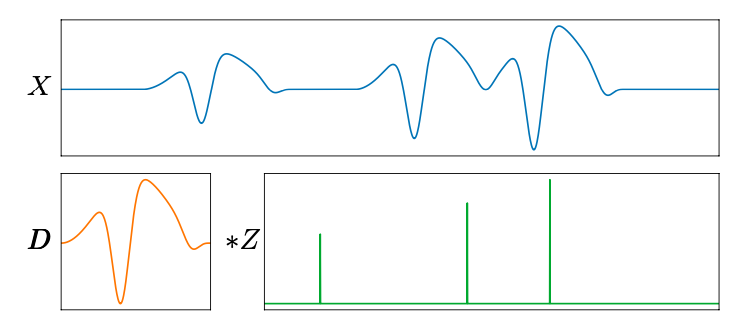
\includegraphics[scale=0.5]{pics/atom_decomposition.png}
    \caption{Decomposition of a noiseless univariate signal $X$ (blue) as the convolution $Z * \boldsymbol{D}$ between a temporal pattern $\boldsymbol{D}$ (orange) and a sparse activation signal $Z$ (green).}
    \source{\cite{moreau2019distributed}}
    \label{fig:signal_decomposition}
\end{figure}

The optimisation problem is as follow\footnote{Note that we are in the case of 1D-convolution, in multivariate CSC.}:
\begin{equation}\label{eq:csc_problem}
\begin{gathered}
\min _{D_{k}, z_{k}^{n}} \sum_{n=1}^{N} \frac{1}{2}\norme{X^{n}-\sum_{k=1}^{K} z_{k}^{n} * D_{k}}_{2}^{2}+\lambda \sum_{k=1}^{K}\norme{z_{k}^{n}}_{1} \\
\text { s.t. } \quad \norme{D_{k}}_{2}^{2} \leq 1 \text { and } z_{k}^{n} \geq 0
\end{gathered}
\end{equation}
where $\braces{X^n}_{n=1}^N \in \R^{P\times T}$ are $N$ observed multivariate signals, $\lambda > 0$ is the regularization parameter, $\braces{D_k}_{k=1}^K \in \R^{P\times L}$ are the spatio-temporal atoms, $\braces{z_k^n}_{k=1}^K \in \R^{\widetilde{T}}$ are $K$ sparse signals of activations associated with $X^n$, with $\widetilde{T} \coloneqq T - L + 1$, and where $z_{k}^{n} * D_{k}$ denotes the convolution between the two signals, obtained by by convolving every row of $D_k$ by $z_k^n$.

In order to better account for the nature of brain signals, a rank-1 constraint is added to the dictionary: $D_k = u_k v_k^T \in \R^{P\times L}$, with $u_k \in \R^P$ being the pattern over channels and $v_k \in \R^L$ over time.
Thus, the $\norme{D_{k}}_{2}^{2} \leq 1$ constraint in \eqref{eq:csc_problem} is now replaced by $\norme{u_{k}}_{2}^{2} \leq 1$ and $\norme{v_{k}}_{2}^{2} \leq 1$.
This rank-1 constraint comes from Maxwell's equations and the physical model of electrophysiological signals like EEG or MEG, where each sensor is supposed to instantly receive a linear transformation of every sources, with a constant topographic map, i.e., a signal coming from the same source at two different times will be spread across the sensors with the same linear transformation.
Thanks to this rank-1 constraint, the learned atoms have a spacial and a temporal pattern, as shown in Figure~\ref{fig:atom_location_and_form}.

\begin{figure}[h!]
    \centering
    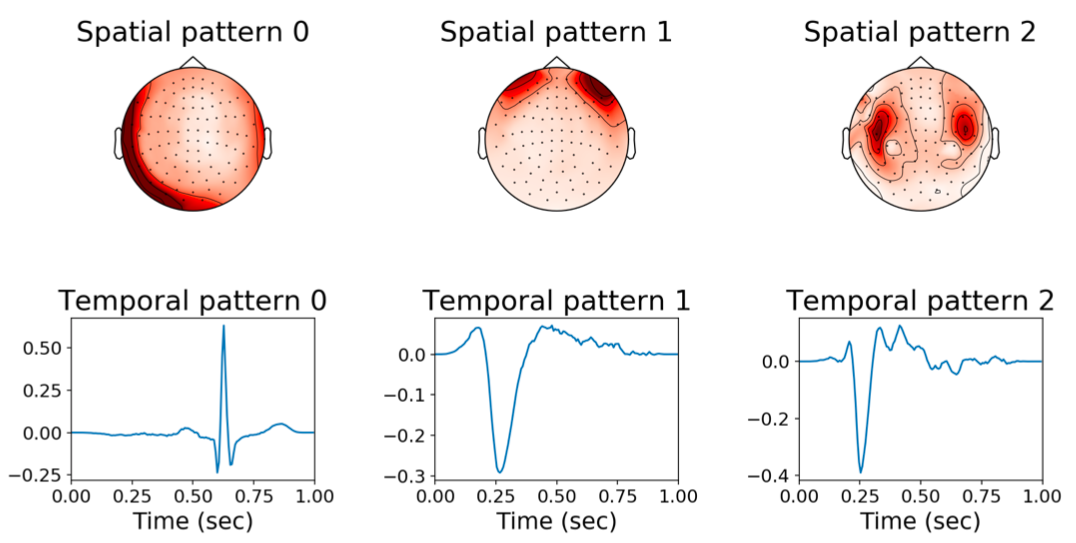
\includegraphics[scale=0.35]{pics/atom_location_and_form.png}
    \caption{Spacial (up) and temporal (down) representation of three atoms obtained by dictionary learning}
    \source{\href{https://alphacsc.github.io/auto_examples/multicsc/plot_sample_evoked_response.html#sphx-glr-auto-examples-multicsc-plot-sample-evoked-response-py}{Example in \texttt{alphacsc} package's documentation}}
    \label{fig:atom_location_and_form}
\end{figure}

In python, the package \href{https://alphacsc.github.io/index.html}{\texttt{alphacsc}} makes it possible to carry out such an operation.
In practice, we do not have $N$ signals, as the brain of every person is different, it would make no sense to consider that the atoms of one subject are strictly identical to another.
Thus, we split the recorded signal $X\in\R^{P\times T}$ into several smaller signals, in order to take advantage of the factorised computations describe in \citep{dupre2018multivariate} that speed up computational time, and eventually to be able to distribute computations \citep{moreau2019distributed}\footnote{Note that distributed CSC is not implemented yet into \texttt{alphacsc}.}.
Once the original signal is split into $N$ smaller signals, the dictionary of atoms $D$ and their associated activations vectors $z_k^n$ are learned.
Finally, an ultimate action is done: with the learned dictionary $D$ and with the original signal $X$, the matrix $z \in \R^{K\times \widetilde{T}}$ is learned solving \eqref{eq:csc_problem}.

%\citep{jas2017learning}:
%\begin{itemize}
    %\item Neural time-series data contain a wide variety of prototypical signal waveforms (atoms) that are of significant importance in clinical and cognitive research. One of the goals for analyzing such data is hence to extract such ‘shift-invariant’ atoms.
    
    %\item convolutional sparse coding (CSC) model for learning shift-invariant atoms from raw neural signals containing potentially severe artifacts.
    
    %\item A natural way to cast the problem of learning a dictionary of shift-invariant atoms into an optimization problem is a convolutional sparse coding (CSC) approach
    
    %\item As opposed to using generic bases that have predefined shapes, such as the Fourier or the wavelet bases, these atoms provide a more meaningful representation of the data and are not restricted to narrow frequency bands.
    
    %\item neural signals often contain heavy noise bursts and have low signal-to-noise ratio.
%\end{itemize}

%Résumé de \cite{dupre2018multivariate}:
%\begin{itemize}
    %\item Frequency-specific patterns of neural activity are traditionally interpreted as sustained rhythmic oscillations, and related to cognitive mechanisms such as attention, high level visual processing or motor control. While alpha waves (8–12 Hz) are known to closely resemble short sinusoids, and thus are revealed by Fourier analysis or wavelet transforms, there is an evolving debate that electromagnetic neural signals are composed of more complex waveforms that cannot be analyzed by linear filters and traditional signal representations.
    
    %\item In this paper, we propose to learn dedicated representations of such recordings using a multivariate convolutional sparse coding (CSC) algorithm. Applied to electroencephalography (EEG) or magnetoencephalography (MEG) data, this method is able to learn not only prototypical temporal waveforms, but also associated spatial patterns so their origin can be localized in the brain.
    
    %\item Dictionary learning is one family of techniques, which consists in learning atoms (or patterns) that offer sparse data approximations.
    
    %\item When working with long signals in which events can happen at any instant, one idea is to learn shift-invariant atoms. They can offer better signal approximations than generic bases such as Fourier or wavelets, since they are not limited to narrow frequency bands.
    
    %\item In this study, we develop a multivariate model for CSC, using a rank-1 constraint on the atoms to account for the instantaneous spreading of an electromagnetic source over all the channels. -> Maxwell equation, thanks to the rank-1 model can be localized in the brain for clinical or cognitive neuroscience studies.
    
    %\item bien expliquer l'hypothèse de rang 1, comme quoi c'est une conséquence de la linéarité et de l'immédiateté des équations de Maxwell. Pour un capteur $x_n$, le signal reçu peut être représenté comme étant $S$ (l'ensemble de tous les signaux) plus un signal $v_k$ (issu d'un dipole dans le cerveau, ici intervient l'immédiateté du signal, il n'y a pas de latence) multiplié par une constante $u_{n,k}$ (ici intervient la linéarité, tous les capteurs reçoivent en même temps le même signal magnétique, à une transformation linéaire près). Ainsi, puisque l'on peut faire de même avec tous les capteurs, on peut représenter les signaux reçu comme étant $X = S + u_k v_k^T$, et ainsi on trouve que $X = \sum_k u_k v_k^T$ (le tout multiplié par un $z_k$, qui lui détermine l'activation dans le temps)
%\end{itemize}